\subsection{Multiplikation von Matrize mit Vektor in CUDA Implimentierung}
Multiplikation der Matrize mal Vektor trefft sehr haufig in wissenschaftliche Rechnen auf. Die Operation kann in unterschiedliche Vektor-Multipliktionen zerlegen.

\subsubsection{Fullmatrizemultiplikation}
Die genaue Implimentierung der Vektor-Multiplikation in CUDA wird folgend (Fig ) gezeigt. Vektor A wird mit Vektor B multipliziert. Man bearbeitet jede Element-Multiplikation in jeweiligem Thread und erzeugt Produktvektor Cs.  Alle Elements von Cs wudern zur ein Skalarwert summiert. Weil CUDA-Blocksize beschrankt ist, [NVIDIA_CUDA_ProgramingGuide_2.3,A.1.1], maximum 512 Threads per Block, muss man f�r gro�e Vektoren in meher Blocks oder ein Block iterativ verwnden.
\begin{firuge}[htbp]
	\centering
	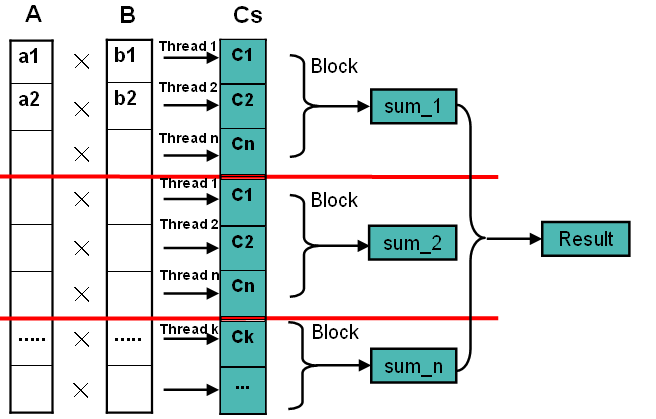
\includegraphics{.//pic//Vektor}
	\caption{Vektor Multiplikation. A : first vector; B:second vector ; Cs: product vector.}
	\lable{fig:vektor}
\end{figure}

Bei der Multipliktionen der Matrizen mit Vektoren ist ganz �nhlich,dass jede zerlegende Vektor-Multipliktion in ein Block bearbeitet wird.

\begin{firuge}[htbp]
\centering
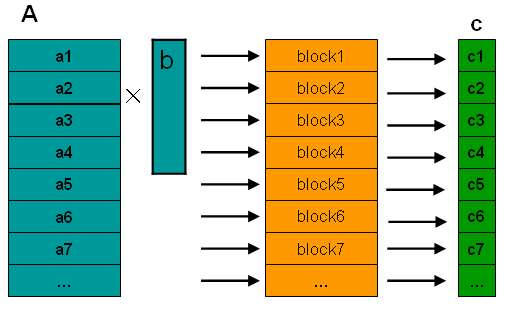
\includegraphics{.//pic//MatrixVektor}
\caption{Matriz mal Vektor. A:Matrize; b: Vektor; c: produkt Vektor}
\lable{fig:vektor}
\end{figure}


\subsubsection{Sparsematrizenmultiplikation}

\subsubsubsection{Sparse-Matrizen}
In vielen Fall bearbeitet man Sparse-Matritzen bei numerische Rechenen. Wie seht eine Sparse-Matrze aus? Wie wird die gespeischert? Fig.1. zeigt auf, wie alle Elements in einer Sparse-Matrize verteilt erden. F�r numerische Speischer wird durch eine einfache Idee nur Nonzero-Elements und zugeh�rige Stelleinfomationen wie in Fig. gespeichert. Der Vektor pr enthalt alle Nonzero-Elements, Vektor ir zugeh�rige Zeileninformationen, Vektor jc Spaltinformationen. Eine weiter kompakte Struktur ist Fig.3. "compressed column structure", indem die Werte von jc[i] und jc[i+1]-1 die Index von zur Spalte i geh�rtet Nonzero-Elements und Zeile aufweisen.

\begin{figure}[htbp]
\centering
\begin{minipage}[t]{0.3\textwidth}
	\centering
	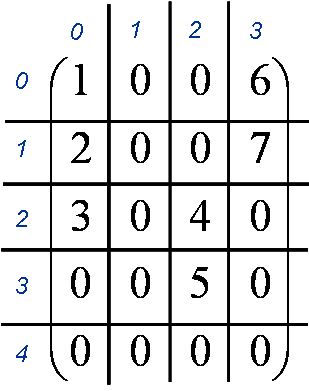
\includegraphics{.//pic//orignal_sparse}
	\caption{Originale-Matrize}
\end{minipage}
\begin{minipage}[t]{0.3\textwidth}
	\centering
	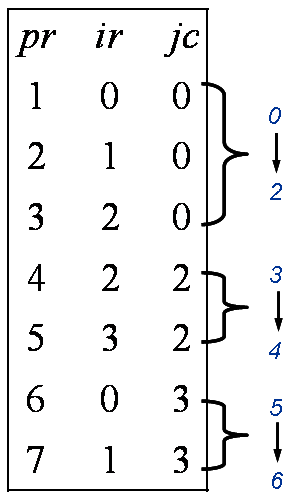
\includegraphics{.//pic//numerische_sparse1}
	\caption{Sparsame Struktur}
\end{minipage}
\begin{minipage}[t]{0.3\textwidth}
	\centering
	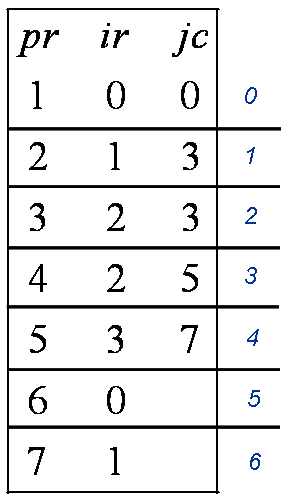
\includegraphics{.//pic//numerische_sparse2}
	\caption{"compressed column structure"}
\end{minipage}	
\end{figure}


\subsubsubsection{SparseMatrixMultiplikation}
In "compressed column structure " wird Sparsematrizen in Spaltfolg gespeichert.  In unser Implementierung verwendt man in Zeilfolg gespeischerte SparseMatrizen. Folgend Fig zeigt die genau Verfahren dieser Operation.  Wie vorliegend beschreibung besteht Sparsermatrix aus 3 Vektoren Pr, Ir, Jc. Aus Jc findet man zu jede Zeile geh�rte Nonzero-Elements und Spalteninfo, die auch  entspreschende Elements aus Vektor b zeigen. Weiter Verfahren ist die Multiplikation der ausgewahlten Nonzero-Elementen  und Elements aus Vektor b, die analog zu Vektormultiplikation.

\begin{firuge}[htbp]
\centering
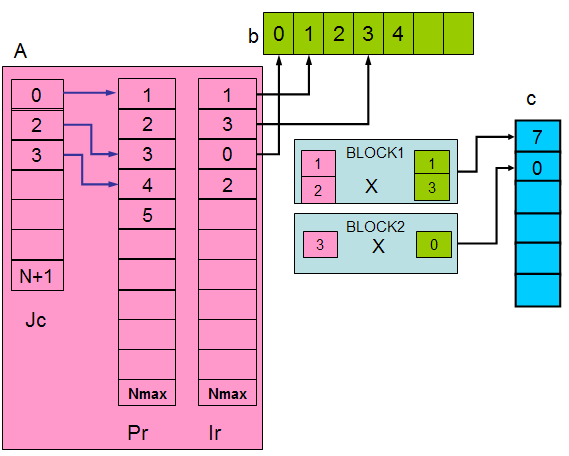
\includegraphics{.//pic//sparseMul}
\caption{Sparsematrizenmultiplikation. A:Sparsematrize, Jc:Vektor der Zeileinfo, Pr: Vecktor der Nonzeroelements, Ir: Vektor der Spalteninfo ; b: Vektor; c: produkt Vektor}
\lable{fig:sparsmultiplikation}
\end{figure}

\subsection{Perfrmance-Optimierung}
Eine weitere �berlegung ist Perfrmance-Optimierung der vorgestellt Operationen in CUDA-Implimentierung. .
Folgend sind audground der Implimentierung der jede Operationen.

1. Dreieckf�rmige Summation (Sumierung in Parallel)
2. Minimierung leer laufende Thread.(32 Thread ein Wrap )
3. Share Memory (geringer latency als globale Memory)

\subsubsection{Dreieckf�rmige Summation}
Aus der Beschreibungen der Operationen Multipliktionen der Matrize mal Vektor und Sparsematrize  mal Vektor beruhen obige Operationen auf Vektormultiplikationen, die anschlie�lichen ein Summierungverfahren in jedem Block enthalten. Blocksummation in einzigen Thread ist nicht effizent. Die einf�hrende Algorithmus: Dreieckf�rmige Summation lautet wie Fig [] . In erstschritte werden 2n und 2n+1 Elements des Produktvektors Cs in jeweilig Threads summiert. In zweiter schritte werden 4n und 4n+2 Elements summiert. Bis BlockSize/2 Schritte erhalt man endlich Ergebnisse.

\begin{firuge}[htbp]
\centering
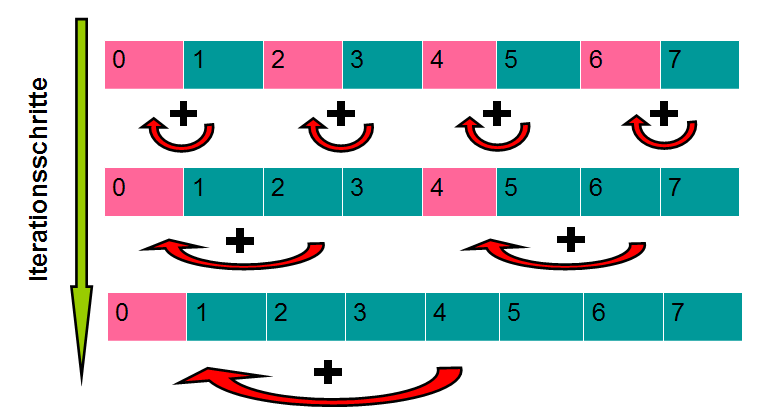
\includegraphics{.//pic//dreieck}
\caption{Dreieckf�rmige Summation. Von Oben nach Unter zeigt}
\lable{fig:Dreieckf�rmige}
\end{figure}

\subsubsection{Minimierung leer laufende Thread}
Im Cuda, bearbeitet jede Multiprzessors gleichzeitig eine Warp von 32 Threads[cuda programing guide], die alle zur selbe Block geh�ren. d.h. F�r sehr d�mm bestzt Matrix, wie in Sparse-Matrix-Multiplikation, sind viele Threads in Leerlauf. Um die Anzahl der in Leer laufende Thread zu minimieren, werden mehre Zeile in eine Block bearbeitet. Dazu verwndet man 2 Dimensionenblocksize. Die Dimension X wird hier f�r Elementemultiplikationen innerhalb jeweiliger Vektormultipliktionen definiert. Die Dimension Y besorget Unterschiedlich Vektormultiplikationen innerhald eines Blockes. Ein optimierte Beispiel ist Sparsermatrizemultiplikation, deren Implimentierung �hnlich obiger Darstellung ist. Wie bestimmt man die genaue Gr��e f�r beide Dimensionen?  Man kann f�r speziale Anwendungen durch Folgende Vesuche die beide Dimensiongr��e auswhalen. Fig[] zeigt die Laufzeit der Multipliktion Ein-Diagonalematrize mal Vektor mit unterschiedliche Blocksize. Es ist offenbar,dass f�r 1-Diagonalmatize das optimale Blocksize 16x1 oder 32x1 betr�gt. 1-Diagonalmatize ist nicht einzige d�nbesetzte Matrize in unser Anwendung. Dickere Sparsermatrizen entstehen auch haufig. Fig[] ist die Messung f�r 32-Diagonalmatize. Man find 16x16 eine schlauere Auswahl.

\begin{figure}[htbp]
\centering
\begin{minipage}[t]{0.3\textwidth}
	\centering
	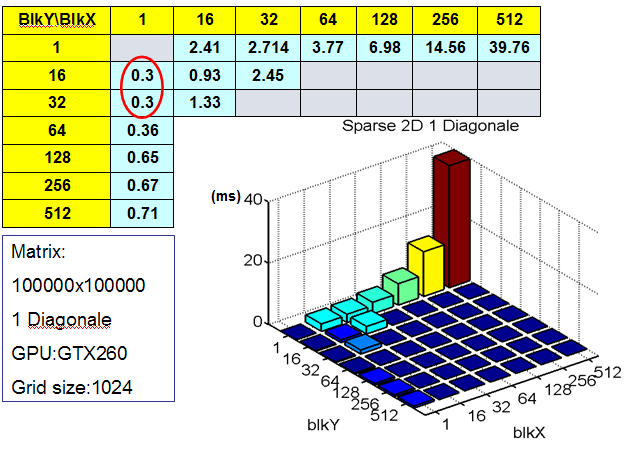
\includegraphics{.//pic//einDiagonal}
	\caption{Multipliktion Ein-Diagonalematrize mal Vektor. BlockY: Anzahl der Y-Dimension von Block; BlockX: Anzahl der X-Dimension von Block}
\end{minipage}
\begin{minipage}[t]{0.3\textwidth}
	\centering
	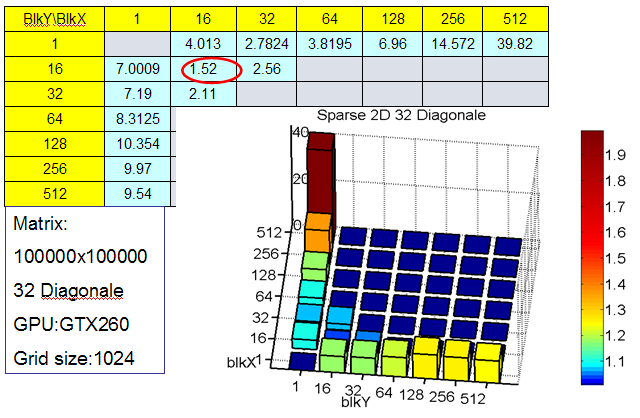
\includegraphics{.//pic//moreDiagonal}
	\caption{Multipliktion 32-Diagonalematrize mal Vektor. BlockY: Anzahl der Y-Dimension von Block; BlockX: Anzahl der X-Dimension von Block.}
\end{minipage}
\end{figure}

Wie effezient ist denn optimierte CUDA-Implimentierung? 
Weiter Versuch der Vergleichung von matlab,CPU-und GPU-Implimentierung wird in Fig[] ausgewiesen. F�r 128-Diagonalmatize kann CUDA-Implimentierung gegen CPU zu Faktor 9 erreichen.
\begin{firuge}[htbp]
\centering
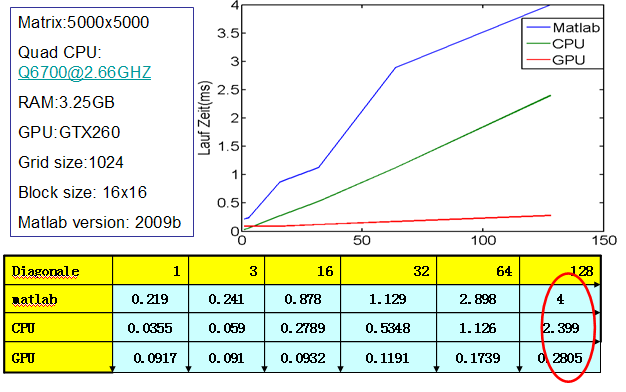
\includegraphics{.//pic//compareSparse}
\caption{Vergleichung der Sparseermatrize-Multiplikation von matlab,CPU-und GPU-Implimentierung.}
\lable{fig:compareSparse}
\end{figure}

\subsubsection{Share Memory}
Im Grafikater ,sind Zugriff der Globalespeicher  langsamer als �nder Speicher.  Wie Beispiele in [CUDA Programing Guide] gezeigt, kann man meher mal verwendete Daten zun�chst in share Memory schreiben, dann f�r die entsprechenden Operationen benutzen. In der Multipliktion der Fullmatrize mal Vektor wird jede Vektorelemnt mehr mal gebraut. Nach Untersuchungen wahlen wir 1-Dimensionblock,die 64 betr�gt und jede Vektorelement 8 mal gerbraucht in einem Block, d.h. in jedem Block 8 zerlegene Vektormuliplikation bearbeitet werden. Aus den Ergebnise von Fig[](Vergleich von optimierte Fullmatrix-Multiplikatin mit C-Implimentierung und alte GPU-Implimentirung f�r MxN Fullmatrizen) 

\begin{firuge}[htbp]
\centering
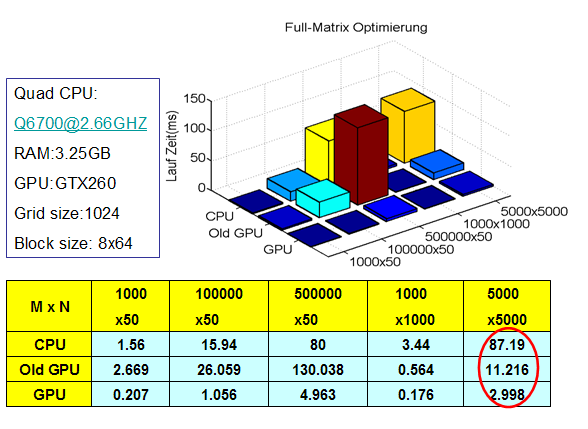
\includegraphics{.//pic//sharememory}
\caption{Vergleich von optimierte Fullmatrix-Multiplikatin mit C-Implimentierung und alte GPU-Implimentirung f�r MxN Fullmatrizen}
\lable{fig:sharememory}
\end{figure}

Die optimierte GPU-Implimentierung ist immer schnelle als die CPU-Implimentierung  und die Alte. F�r Matrize 5000x500 kann die CUDA-Program 30 mal schneller als CPU.